\newpage
\section*{Location TUM}

\vspace{2cm}
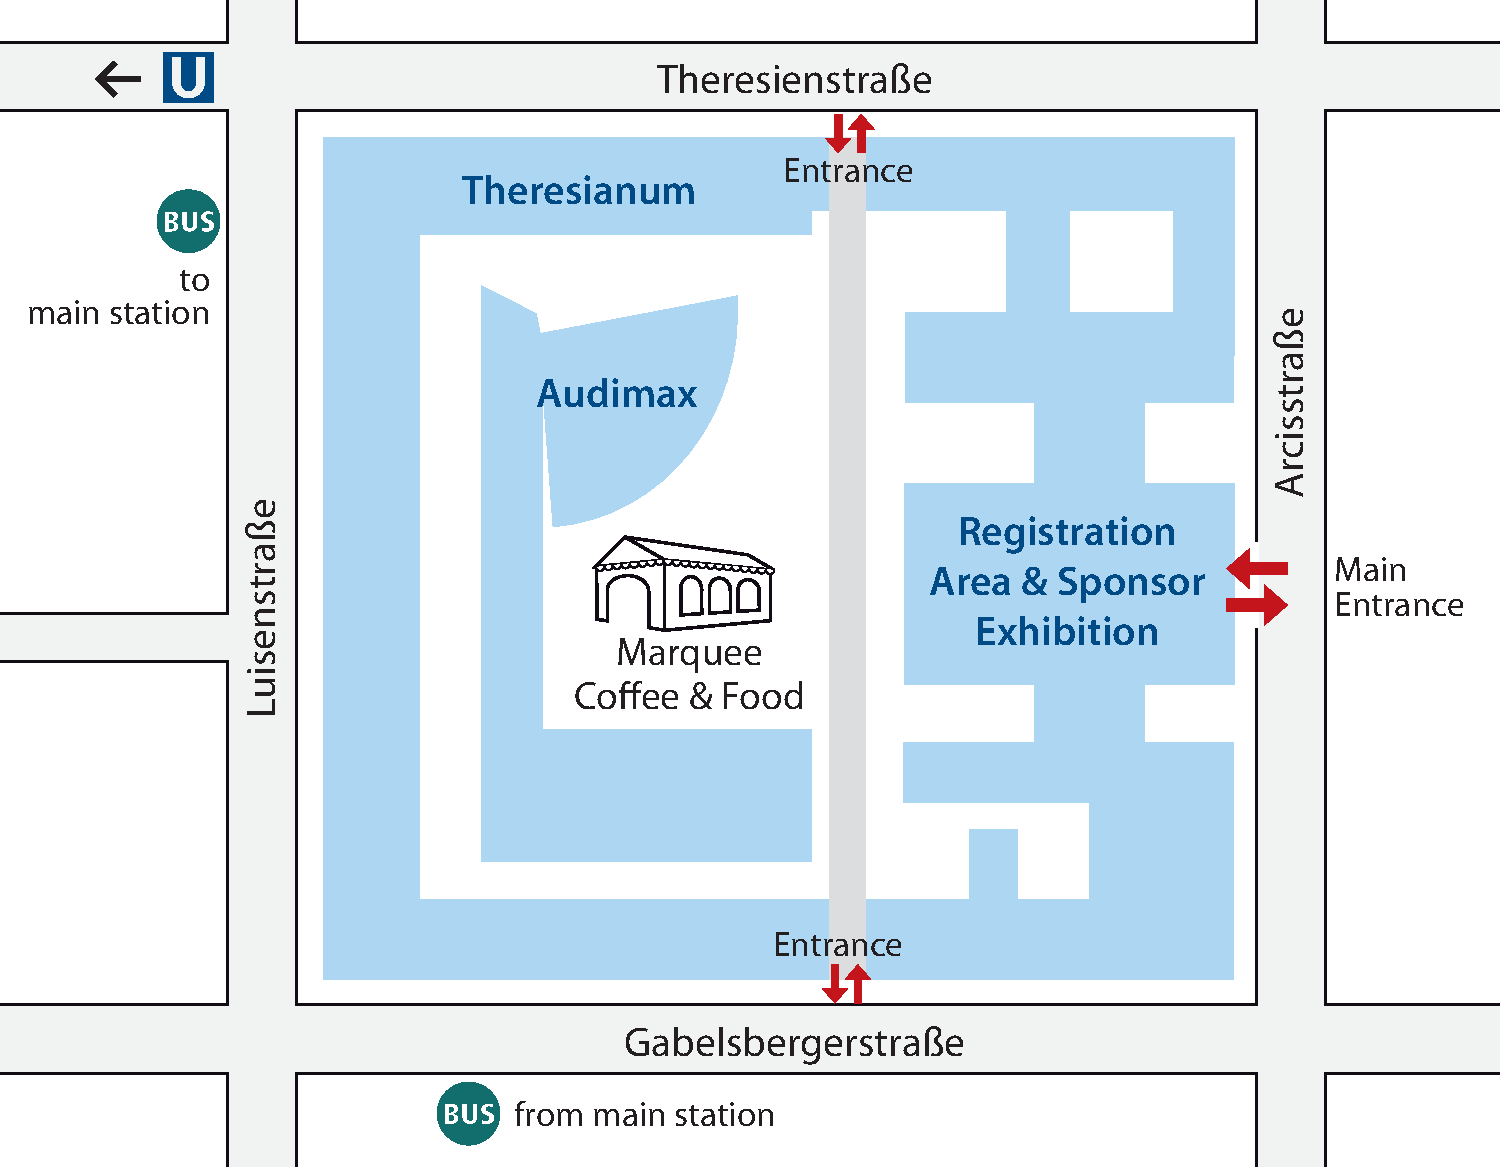
\includegraphics[width=\linewidth]{images/Gelaendeplan_TUM_V2.pdf}

\newpage
\section*{Lecture Halls in the Theresianum}

\vspace{2cm}
% \fbox{
    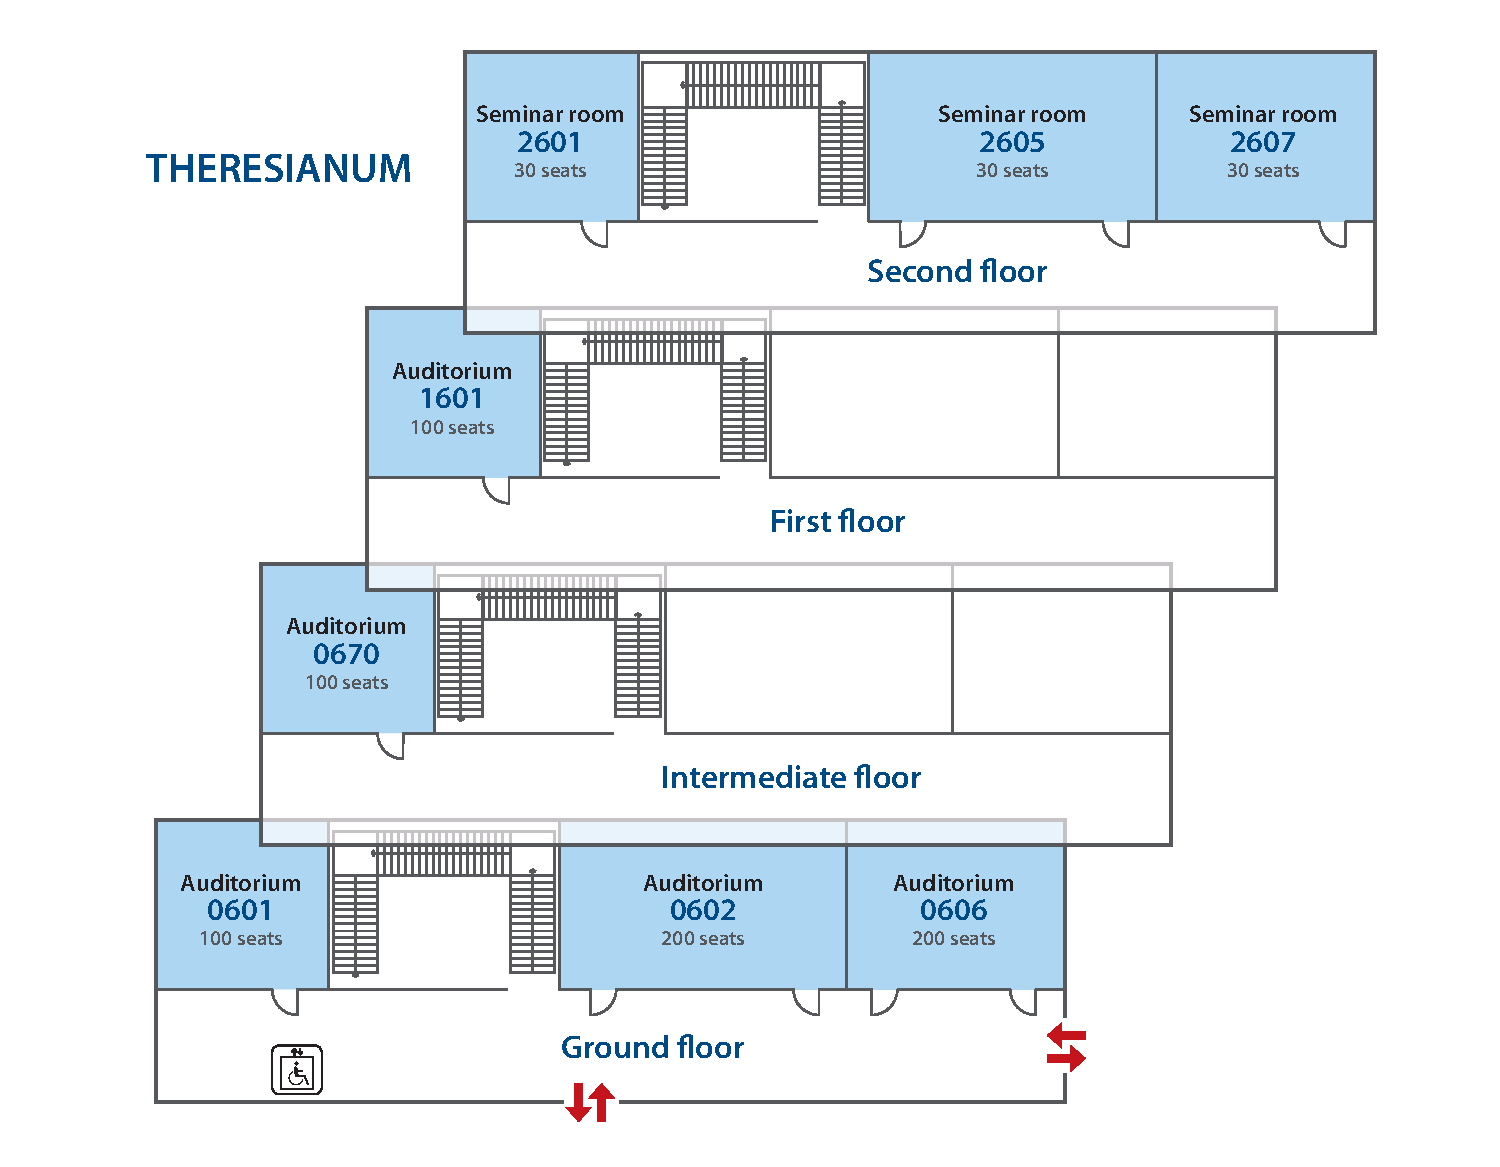
\includegraphics[width=\linewidth, trim=15mm 0mm 15mm 0mm, clip] {images/Raumplan_Theresianum_V2.pdf}
% }

\newpage
\section*{Street Map}

\begin{tabular}{lr}
\begin{minipage}{55mm}
\textbf{Conference Location (A)} \\
TUM, Arcisstraße 21 \\
\textbf{Reception (1)} \\
Old Town Hall, Marienplatz 15 \\
\textbf{Banquet (B)} \\
Hofbräuhaus, Platzl 9
\end{minipage}
&
\begin{minipage}{20mm}
\includegraphics[width=20mm]{images/qrcode.pdf} 
\end{minipage}
\end{tabular}

\vspace{5mm}
\includegraphics[width=\linewidth]{images/map.png}

{\tiny Map data (c) OpenStreetMap contributors}

\newpage
\section*{Social Events}

Both social events are close by the central place in Munich (Marienplatz).
You can either walk there as shown on the map (2.5 km, about 30 min), or
take public transport.

Public transport options:
\begin{itemize}
 \item bus 100 (leaves from Gabelsbergerstraße, south entrance of TUM, direction Ostbahnhof) to Odeonsplatz. There, switch to the subway U3 or U6 towards Marienplatz (1 stop).
 \item live routing: \url{https://goo.gl/1T1Sg6}
\end{itemize}

\vspace{2mm}
The \textbf{Old Town Hall} is next to the Marienplatz, 50m to the east. It is a white building (\url{https://goo.gl/XE2OUV}), not to be confused with the large, red New Town Hall
immediately next to the Marienplatz.

\vspace{2mm}
The \textbf{Hofbräuhaus} (\url{https://goo.gl/SUUQvW}) is a few minutes east and north of the Marienplatz, as shown on the map. Turn left behind the Old Town Hall into Sparkassenstraße, right into Münzstraße, and left into Platzl.
